% $Id: theory.tex 142 2012-12-22 10:41:32Z danbos $
\chapter{Development of Modern Web Applications}
\label{ch:theory}
\noindent
When developing in a modern context, in particular for the Internet, one needs to
understand how to develop securely, efficiently and without repeating oneself. Though not as much is needed to understand the pertinent areas that this course covers, they are still important to understand the broader strokes.

\section{Separation of Concerns}
\label{sec:architecture}
\noindent
Per \citep{Wikipedia2013} Multitier architecture is a ``client–server architecture in which presentation, application processing, and data management functions are logically separated''. In Web Development, that is most commonly generalized to three tiers:

\subsection{Frontend}
\noindent
What is actually served to the browser, whether it's dynamically generated or static. It includes JavaScript, CSS, HTML, typography, graphics, etc. The user interface, or presentation layer. In this system, the least concerns have been put into the frontend, excepting details needed to show understanding of JavaScript-based security issues.

\subsection{Middle}
\noindent
What is most commonly referred to as ``web development'', be it in Ruby on Rails, PHP,
.NET or any other kind of server-side languages. The bulk of this system is written in PHP,
using the framework Laravel.

\subsection{Backend}
\noindent
Where the middle processing technologies generate the frontend consumed by the browser, in most dynamic systems it gets its' information -- data -- from the backend database or data store, whether through a MySQL database, a NoSQL MongoDB or any other kind of system, the backend provides access to the data, and should be properly secured.

\section{Technologies}
\label{sec:technologies}
\noindent

Termer och förkortningar som är viktiga för läsarens förståelse av den 
fortsatta framställningen förklaras i detta kapitel.
Första gången du i den löpande texten använder ett begrepp eller en förkortning 
ska du förklara det, även om det dessutom finns definierat i ett 
terminologiavsnitt.
När begrepp introduceras skrivs de med emfas.

Första gången en \emph{förkortning} (förk.) används skrivs den inom parentes 
efter dess förklaring, såsom exemplifieras i denna mening.

Använd svenska termer så långt det är möjligt.
Se Svenska datatermgruppens \citep{Datatermgruppen} rekommendationer på URL
\begin{center}
	\url{http://www.datatermgruppen.se/}.
\end{center}


\section{Att referera eller citera}
\label{sec:ref}
\noindent
Du refererar när du sammanfattar eller återger en text med egna ord.
Exempelvis:
Forsslund förespråkar mer berättande rubriker i tekniska rapporter och menar 
att man särskilt i underrubrikerna kan ge viktig information 
\citep{Forsslund1969raf}.

Du citerar när du ordagrant återger en fras, en mening eller ett stycke.
I normalfallet refererar man istället för att citera källor.
Du kan använda direkta citat om du har speciella skäl, till exempel om du vill 
återge vedertagna definitioner av begrepp, när du tycker att en författare 
formulerat sig på ett särskilt träffande sätt, när du behöver stöd av en 
auktoritet, eller när du vill visa att en författare har fel.

Korta citat omges med citationstecken.
Att citera Strömqvist kan vara en passande illustration i detta sammanhang:
''Det må vara svårt att skriva, men det är roligt också.'' \citep[sidan 
X]{Stromquist2000s}.

Långa citat kan återges i form av blockcitat.
Textmassan placeras då på sidan utan citationstecken, men med indrag, det vill 
säga något förskjutet åt höger, och med mindre teckenstorlek.
Källan anges i direkt anslutning till citatet.
\begin{quote}
	Det här är ett blockcitat vilket innebär indragning, mindre teckenstorlek, 
	rak vänstermarginal, inte nödvändigtvis rak högermarginal, och inga 
	citationstecken.
	Blockcitatet kan tillämpas vid mer än ungefär 50 ord.  Blockcitat avslutas 
	alltid med källhänvisning. \citep[sidan X]{Stromquist2000s}
\end{quote}

\subsection{Testing}
\noindent
\dots
Se \prettyref{sec:aim} \dots
Se också \prettyref{ch:introduction} \dots


\section{Källhänvisningar och -förteckning}
\label{sec:references}
\noindent
Att kopiera in en text utan att ange dess källa betraktas som plagiat och 
därmed allvarligt fusk.

En källförteckning (lista över referenser) upprättas i slutet av rapporten för 
att ge läsaren en samlad upplysning om samtliga källor som du refererar, 
citerar eller av annat skäl hänvisar till i den löpande texten.
Källor ska anges så noggrant att läsaren ska kunna kontrollera dem, om de finns 
tillgängliga via bibliotek eller på internet.
Det förekommer även att muntliga källor och annan korrespondens inkluderas 
i källförteckningen, men det är ovanligt i tekniska rapporter.

Använd vederhäftiga källor, gärna författade av auktoriteter på området.
Privata hemsidor och studentuppsatser har låg tillförlitlighet som källor, 
i synnerhet om studentuppsatsen har lägre nivå (A, B, C eller D) än det egna 
arbetet.
Var källkritisk, särskilt mot kommersiella försäljningsargument.

Ta endast med källor i förteckningen som du refererar eller citerar i den 
löpande texten, detta sker automatiskt i \LaTeX och Bib\TeX.
Samtliga källor som tas upp i källförteckningen ska vara kopplade till 
rapporten genom hänvisning i den löpande texten, enligt Vancouver-systemet, som 
är vanligt förekommande i rapporter i tekniska ämnen.

Enligt Vancouver-systemet ordnas källförteckningen i den ordning källorna 
återges i den löpande texten, och källhänvisningen anges i texten med en siffra 
inom hakparenteser, som i detta dokument.
% De anges även i denna ordning i källförteckningen.
Exempel på källhänvisning:
Enligt \citet{Eriksson2001dsf} kan dynamiska SFN ge betydande prestandavinster.
På liknande sätt refereras till källor på internet, exempelvis kan du se 
\citet{Wikipedia2010h264} för att läsa om \emph{H.264}.

Eftersom information på webben kan revideras ofta, och eftersom webblänkar kan 
upphöra att fungera, måste datum anges då du själv hämtade information från 
webbsidan.
Vid webbaserade källor krävs ibland anvisningar för hur källan kan hittas. Tänk 
på att kvaliteten på materialet på internet varierar.


\section{Illustrationer}
\label{sec:illustrations}
\noindent
Samtliga illustrationer (bilder, figurer, diagram, tabeller) i rapporten ska 
vara numrerade och försedda med en kort figur- eller tabelltext.
Därtill ska i anslutning till texten anges källhänvisning varifrån 
illustrationen är hämtad, om den inte är av egen produktion.
Se \prettyref{fig:automata} för ett exempel.

\begin{figure}
	\centering
	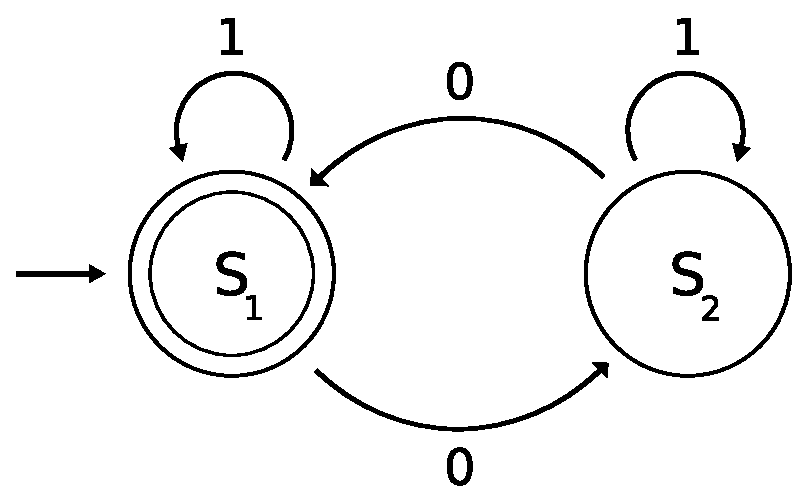
\includegraphics[width=7cm]{automata.eps} % for latex(1)
	% 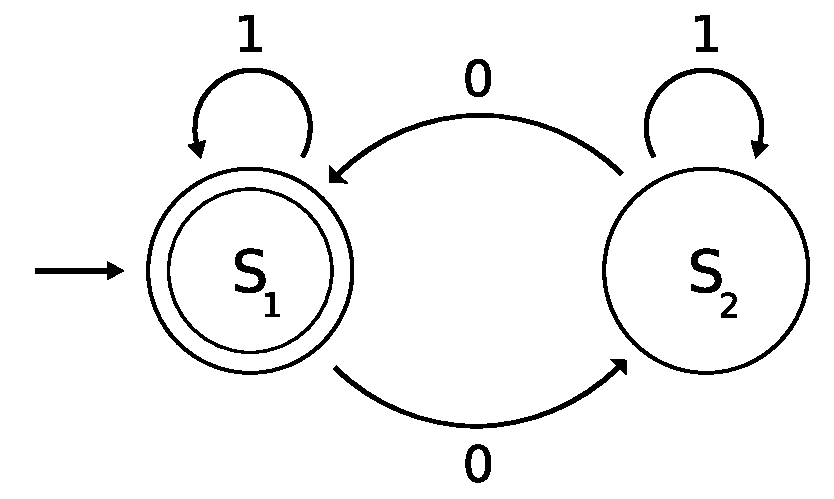
\includegraphics[width=7cm]{automata.pdf} % for pdflatex(1)
	\caption[Ett exempel på en automat.]{Ett exempel på en automat 
	\citep{Wikipedia2012at}.}
	\label{fig:automata}
\end{figure}

Samtliga illustrationer ska vara kopplade till rapporten genom hänvisning i den 
löpande texten.
Hänvisningarna skrivs på svenska med begynnande gemen, likt den ovan.
På svenska skrivs figur alltid med inledande gemen då de förekommer i löpande 
text.

\begin{table}
	\centering\small
  \begin{tabular}{r|cccccccccc}
    \hline\hline
    \(\alpha\) & a & b & c & d & e & f & g & h & i & j \\
    \(P_E(\alpha)\) & 8.2  & 1.5 & 2.8 & 4.3 & 12.7 & 2.2 & 2.0 &
    6.1 & 7.0 & 0.2 \\
    \(P_S(\alpha)\) & 9.3  & 1.3 & 1.3 & 4.5 & 9.9 & 2.0 & 3.3 &
    2.1 & 5.1 & 0.7 \\
    \hline\hline
    \(\alpha\) & k & l & m & n & o & p & q & r & s & t \\
    \(P_E(\alpha)\) & 0.8 & 4.0 & 2.4 & 6.7 & 7.5 & 1.9 & 0.1 & 6.0 & 6.3 &
    9.1 \\
    %\(P_S(\alpha)\) & 3.5 & 8.8 & 4.1 & 1.7 & 0.007 & 8.3 & 6.3 & 8.7 &
    \(P_S(\alpha)\) & 3.2 & 5.2 & 3.5 & 8.8 & 4.1 & 1.7 & 0.0 & 8.3 & 6.3 &
    8.7 \\
    \hline\hline
    \(\alpha\) & u & v & w & x & y & z & å & ä & ö \\
    \(P_E(\alpha)\) & 2.8 & 1.0 & 2.4 & 0.2 & 2.0 & 0.1 & 0.0 & 0.0 & 0.0 \\
    \(P_S(\alpha)\) & 1.8 & 2.4 & 0.03 & 0.1 & 0.6 & 0.02 & 1.6 & 2.1 &
    1.5 \\
    \hline\hline
  \end{tabular}
	\caption[Tabell av sannolikhetsfunktionen för bokstäver i det engelska 
	respektive svenska språket.]
	{Tabell av sannolikhetsfunktionen för bokstäver i det engelska och det 
	svenska språket, \(P_E\) respektive \(P_S\), angiven i procent med en 
	decimals noggrannhet \citep{Wikipedia2011lf}.}
  \label{tbl:freq}
\end{table}

Se \prettyref{tbl:freq} för ett exempel på en tabell.
Automatisk numrering fungerar på samma sätt som för figurer, titeln kommer dock 
automatiskt att vara tabell istället för figur.
Att Referera till tabeller i texten följer samma regler som för figurer och 
utförs på samma sätt.


\section{Matematiska formler}
\label{sec:maths}
\noindent
Ett exempel på hur matematik bör formuleras i skrift ges i följande meningar.
Låt \(a\) och \(n\) vara heltal sådana att \(\gcd(a,n) = 1\), det vill säga att 
\(a\) och \(m\) är relativt prima.
Då har vi att
\begin{equation}
	\label{eq:fermat-euler}
	a^{\varphi(n)} \equiv 1 \pmod n,
\end{equation}
där \(\varphi\) är Eulers \(\varphi\)-funktion.
Resultatet i \prettyref{eq:fermat-euler} är känt som Fermat-Eulers sats.

Ytterligare ett exempel:
Den effekt \(P_{i,j}\) som överförs från en basstation \(i\) till mobiltelefon 
\(j\) modelleras enligt
\begin{equation}
	\label{eq:power}
	P_{i,j} = C\cdot \frac{P_i G_{i,j}}{d^\alpha_{i,j}},
\end{equation}
där \(P_i\) är basstationens sändareffekt; \(d_{i,j}\) är avståndet mellan 
basstationen och mobiltelefonen; \(\alpha\) är en utbredningsexponent som är 
\(2\) i fri rymd och cirka \(3\) till \(4\) i stadsbebyggelse; \(C\) är en 
faktor som beror av antennförstärkning, kanalfrekvens och antennhöjd; samt 
\(G_{i,j}\) är en stokastisk variabel som återspeglar fädningens inverkan.
Utifrån \prettyref{eq:power} inses att den mottagna effekten är proportionerlig 
mot sändareffekten.

Ibland kan en ekvation eller härledning behövas delas upp på flera rader, likt 
ekvationerna \eqref{eq:basecase} och \eqref{eq:recursion}.
\begin{quotation}
	When the message-blocks \(M_i\) are processed, it is done accordingly:
	\begin{eqnarray}
		\label{eq:basecase}
		H_0 &=& G, \\
		\label{eq:recursion}
		H_{j+1} &=& E(H_j, T_j, M_j),
	\end{eqnarray}
	where \(T_j\) is the tweak-value with the bit-fields set correctly for the
	\(j\)th block. When all blocks are processed, the final \(H\) is the result 
	of the UBI chaining mode.
	This means that each block is processed uniquely, they all depend on each 
	other and the original message has now been compressed to a single 
	block-sized result.
\end{quotation}

Det är dock inte alltid nödvändigt att numrera ekvationerna, exempelvis om vi 
bara nämner summan mellan \(1\) och \(100\),
\begin{equation}
	\nonumber
	\sum^{100}_{i=1} i,
\end{equation}
utan att senare referera till den behövs ingen numrering.
